\documentclass[11pt, a4paper]{report}
\usepackage[utf8]{inputenc}
\usepackage{float}
\usepackage{array}
\usepackage{amsmath}
\usepackage{amssymb}
\usepackage{amsfonts}
\usepackage{latexsym}
\usepackage{graphicx}
\usepackage{tabularx}
\usepackage{ltxtable}
\usepackage{longtable}
\usepackage{color, colortbl}
\usepackage{caption}%\usepackage{subcaption}
\usepackage{ifpdf}
\usepackage[hidelinks]{hyperref}
\usepackage{url}
\usepackage{xtab}
\usepackage[hmargin=3cm,vmargin=3cm]{geometry}
\usepackage[norsk]{babel} 
\usepackage[parfill]{parskip}
\usepackage{pdfpages}
\usepackage{listings}
\usepackage{subfigure}
\usepackage{xcolor,colortbl}

% Begin chapter numbering
\usepackage[T1]{fontenc}
\usepackage{titlesec, blindtext, color}

\definecolor{gray75}{gray}{0.75}
\newcommand{\hsp}{\hspace{20pt}}
\titleformat{\chapter}[hang]{\Huge\bfseries}{\thechapter\hsp\textcolor{gray75}{|}\hsp}{0pt}{\Huge\bfseries}
% End chapter numbering

% Add numbering to subsubsection
\setcounter{secnumdepth}{3}
\setcounter{tocdepth}{3}

\definecolor{Gray}{gray}{0.9}

% Header packages
\usepackage{fancyhdr}
\pagestyle{fancy}
\rhead{Chapter: \thechapter}

% Custom 
%\newcommand{\newCommandName}{text to insert} % Defines a variable in LaTeX
\newcommand{\comment}[1]{} \comment{This is a block comment wrapped in curly brackets}
%\renewcommand{\thefootnote}{\roman{footnote}}

\begin{document}
%\pagecolor{yellow!30} % Uncomment for debugging floats
\pagenumbering{gobble}


\begin{titlepage}
\begin{center}
\vspace*{1in}
{\LARGE Eksperter i Team}
\par
\vspace{1cm}


\begin{figure}[ht!]
\centering
%
\includegraphics[width=25mm]{images/logo.png}
%\caption{A simple caption}
\label{overflow}
\end{figure}


{\LARGE Stereo}
\par
\vspace{0.6in}
{\LARGE Project report}
\par
\vspace{0.2in}
{\Large Group 1}
\par
\vfill
\par
\vspace{0.5in}
Our names\\ \ldots here\\
\par
\vspace{0.4cm}
\today
\end{center}
\end{titlepage}

%\newpage
%
%\input{section/abstract}

\tableofcontents
\newpage
\pagenumbering{arabic}

\comment{ Struktur:
			Innledning
				Intro til faget
				Introduksjon til gruppa
			Cases
				Holdninger til prosessarbeid
				Avsporing
					Lederløst team
				Overkjøring i diskusjon/oppdeling i delgrupper
				Lunch
			Hva har vi lært av casene?
}
%%%
% Put new includes here
%%%

\chapter{Introduksjon}
\section{Gruppen} 
\subsection{Emil Bjørlykhaug}
Går undervannsteknologi, 2-årig master. Har tidligere gått Automasjon ved Hials.
Som folk flest hadde jeg hørt en del snakk om EiT på forehand, noe positivt, noe negativt. 
Jeg hadde ikke noen store forventninger ang. selve prosjektet vi skulle gjennomføre,
 men hadde en del forventninger til det å jobbe i gruppe, og å lære hvordan gruppedynamikk 
fungerer sett fra både et teoretisk og praktisk perspektiv. Jeg har tidligere selv jobbet 
en del i grupper, men oftest har medlemmene av desse gruppene vært folk jeg har kjent 
fra før. I et tilfelle når jeg studerte på Hials hadde foreleser ansvaret med å dele opp gruppe, 
så jeg havnet på en gruppe med bare ukjente personer. Jeg følte dette er en god måte å 
utfordre folk sosialt, og følte jeg i løpet av semesteret ble utrolig godt kjent med de jeg 
måtte jobbe sammen med.
Jeg er ikke av typen som roper høgest i diskusjoner, og kan ofte bli litt passiv i 
gruppesammenhenger om jeg ikke føler jeg har noe å stille med, men håper 
EiT kan gjøre meg til et bedre gruppemedlem. Jeg er positivt innstilt til faget 
og håper på høgt læringsutbytte.

\subsection{David Hovind} Jeg har ikke hørt så mye om EiT fra før så jeg vet ikke helt hva det går ut på. 
Jeg har derfor et åpent sinn til faget og ser på det som en positiv utfordring. 
Som regel så foretrekker jeg ikke gruppearbeid fordi man blir avhengig av alle andre i gruppen og de blir avhengige av deg. 
Av den grunn så liker jeg best å jobbe selvstendig, siden det finnes mange forskjellige typer mennesker og man vet aldri 
hvilke typer mennesker man havner på gruppe med. Jeg forventer å bli bedre til å kjenne meg selv og få litt innsikt i 
hvordan det er å reflektere over gruppearbeidet.

\subsection{Kristoffer Løvall}
Jeg fikk høre litt forskjellig om Eksperter i Team før dette semesteret, men har 
prøvd å holde de negative holdningene til faget ute. Jeg starter semesteret 
derfor semesteret med en positiv innstilling, spesielt siden landsbyens tema 
virker veldig interessant og spennende. Jeg forventer at det blir lærerikt å 
jobbe på tvers av fagfelt og interesser, og at tverrfagligheten bidrar til å 
designe et godt produkt. På grunn av tidligere gruppearbeid i forhåndsbestemte 
grupper med ukjente personer har jeg ikke store forventninger til det sosiale, 
noe som på sitt vis kan være positivt ettersom det da ikke er mye som skal til 
for at dette går over forventning. Jeg har også jobbet relativt mye i grupper 
gjennom porsjekter både på NTNU og Høgskolen i Bergen, der jeg ofte har endt opp 
med å ta ansvar og fungere som en gruppeleder. Jeg vet også at jeg kan bli noe 
kontrollerede når jeg blir veldig engasjert og brenner for noe.  Målet mitt for 
Eksperter i Team er å "prøve noe nytt" og være litt mer tilbakeholden på denne 
fronten, prøve å jobbe på linje med alle andre uten å "ta over" for noen og 
kontrollere alle detaljer. Jeg vil bli enklere å jobbe i team med og lære meg 
selv å godta andres løsninger og akseptere disse som de beste løsningene, selv om 
min opprinnelige tanke var noe helt annet. Når det gjelder det faglige håper jeg 
alle har høye forventninger både når det gjelder engasjement for å ende opp med 
gode løsninger, samt det å få en god karakter i faget.
\chapter{Tema 1: Lunsj}

%% Skriv om?

Det første temaet vi presenterer omhandler en avtale om felles lunsjpause og hvordan dårlige avtalerutiner og svekket kommunikasjon førte til en situasjon. I starten av EiT kjente ingen av gruppemedlemmene hverandre, det ble derfor enighet om å tilbringe lunsjpausene sammen for å bli bedre kjent med hverandre uten å prate om oppgaven. I alle grupper finnes det normer, der normene bestemmer hvordan gruppemendlemmene skal oppføre seg, eller ikke oppføre seg. \cite{Artikkel2} I en situasjoner der personer ikke kjenner hverandre finnes det utallige normer om hvordan man skal oppføre seg ovenfor hverandre. Det kan anses som normalt å være litt tilbaketrukken for så å vise mer og mer av sin egen personlighet etterhvert som man ser hvordan de andre personene i gruppen reagerer på utspill og meninger. I denne situasjonen viste det seg at disse normene førte til at meninger og følelser ikke ble ytret, men kom fram under gjeldende dags refleksjoner

\section{Situasjonsbeskrivelse}

Under en samtale i oppstartsfasen av faget der vi planla samarbeidet og hvordan vi ville utføre teamarbeidet, ble det gjort en avtale om at vi burde holde sammen i lunsjpausen.

%Prosessteori om hvordan samholdet i gruppen påvirker arbeidet

Temaet ble tatt opp som en situasjon vi burde reflektere over på landsbydag 4 da Nina ikke deltok på felles lunsj. På dette tidspunktet var det flere av gruppemedlemmene som ikke husket eller var klar over at dette var en avtale. Ved enkelttilfeller vil ikke dette ha noe særlig betydning, men kan få konsekvenser dersom et eller flere av gruppemedlemmer ikke deltar på fellesj lunsj gjentatte ganger. Konsekvenser kan da være at man ikke blir så godt kjent med hverandre og at samholdet i gruppen svekkes. 

\subsection*{Refleksjoner og aksjoner}

Da denne situasjonen ble tatt opp var det helt klart at det kom som en overraskelse på Nina. Hun følte selv det var dårlig gjort av henne, og beklaget ovenfor oss andre at hun hadde stukket av uten frovarsel. Vi lærte at beskjeder og avtaler burde være tydelige, slik at alle får de med seg og har en felles forståelse av avtalen. Det var også viktig for oss andre å ytre at dette helt klart ikke var Ninas feil, og at kommunikasjonssvikt var problemet, ikke henne. 

\begin{quote}``
Jeg var ikke klar over at vi hadde en avtale om felles lunsj, men hadde uansett tenkt å spise lunsjen ved gruppebordet.
''\end{quote} \rightline{{\rm --- Erlend}}

Det var helt tydelig at flere hadde samme oppfatning som Erlend og det ble derfor ytret et forslag om å innføre en avtale som også skulle skrives inn i en revidert samarbeidsavtale. At Nina ikke deltok på lunsjen denne dagen ble oppfattet forskjellig av gruppemedlemmene. Noen mente hun var irritert eller hadde en dårlig dag og derfor trakk seg unna for ikke å påvirke oss andre, mens andre var redd hun mislikte gruppen og derfor ikke ville tilbringe fritiden sin med disse gruppemedlemmene. På grunn av disse forskjellige tolkningene av situasjonen ble det diskutert i hvilken grad avtalen skulle bli håndhevet i særsituasjoner. 

\begin{quote}``
Man kan vel egentlig ikke tvinge noen til å gjøre noe de ikke har lyst til. Det er bedre å ta tid for seg selv enn å sitte å lage dårlig stemning, men for å prøve å skape et bedre sosialt samhold i gruppen er det flott om vi kan få til en felles rutine på pausene.
''\end{quote} \rightline{{\rm --- Kristoffer}}

Vi ble enige om at det skulle skrives inn i samarbeidsavtalen som et punkt, men at det skulle være lav terskel for å gi "godkjenning" for at en person er fraværende. Vi forstod at en felles pause var nokså viktig, ikke bare for det sosiale, men også for strukturen i arbeidet. Vi merket at vi ble flinkere og flinkere på å planlegge denne ettersom tiden gikk, og opprettet en ordning der vi bestemte oss for når og hvor vi skulle ha lunsjpause under morgenmøtet. Vi mente også det ville være gunstig å spise lunsj i et annet lokale enn der vi jobbet, for å kunne skille mer mellom arbeid og pause.

% Trenger meeeeeeeeeeer

\section{Evaluering av aksjon} 

Vi ble enige om at vi burde planlegge på starten av dagen et tidpunkt for en felles lunsjpause. Det skaper et godt samhold i gruppa å ha en felles pause.  Da vi skulle revidere samarbeidsavtale la vi derfor til følgende regel:  ``Hver morgen bestemmes et tidspunkt og tidsrom for felles pause.'' Denne regelen ga rom for tolkning når det gladt hvorvidt det var \emph{krav} til å være med på denne pausen, slik at man kunne spørre om å trekke seg unna om nødvendig. I tillegg kan være vanskelig å skille mellom arbeid og pause, og vi kom derfor til enighet om å konsekvent spise i et annet lokale for å skape et klarere skille. Disse tiltakene har vist seg å fungere godt, og vi har som regel vært samlet etter dette, med unntak av sykdomsfravær og lignende. Gjennom det videre sammarbeidet i faget, har vi merket at det sosiale samholdet fikk en bratt opptur etter at denne regelen ble innført. En dag der Erlend og Nina var fraværende ble det reflektert rundt lunsjpausen igjen.

\begin{quote}``
Opplevde det som positivt at vi klarte holde alle som var til stede sammen under lunsjen, spesielt fordi vi var såpass få tilstede på EiT i dag. Det var flere ting jeg merket meg med dagens lunsj. Det å komme seg ut av realfagsbygget (vi spiste på Hangaren) gjorde at det føltes mer som et skikkelig avbrekk enn det tidligere har gjort. Det føltes også lettere enn normalt å holde praten i gang, noe jeg tenker kan være fordi vi er en mindre gruppe. Dette med gruppestørrelser og samhold ble også nevnt i gjennomgangen av prossessartiklene fra EiT-kompendiet tidligere på dagen, og jeg merket at selv om både Nina og Erlend såklart ble savnet under lunsjen, er det lettere å forholde seg til 3 andre enn 5 andre under arbeidet.
\end{quote} \rightline{{\rm --- Kristoffer}}

Som refleksjonen over viser har vi i noen tilfeller også lagt merke til hvordan gruppestørrelsen påvirker både hvordan vi jobbet sammen, og hvordan vi sosialiserte sammen. Kristoffer sier at det var lettere samarbeide og forholde seg til de andre de dagene teamets representanter var få. Dette går inn på et begrep som er kjent innen et team, og som er en definerende faktor for et team, nemlig relasjoner. 
En relasjoner er en forhold mellom to personer og å opprettholde gode relasjoner mellom mange personer samtidig
kan være vanskelig. Et team på seks personer er i følge teorien  \cite{Artikkel4} et litt forstort team med tanke på antallet relasjoner
blant dens medlemmer. Det må derfor jobbes bra med å holde gode relasjoner for dersom én relasjon svikter kan det få 
konsekvenser for hele teamet. 

\begin{quote}``
Teorien sier at grupper på 6 og oppover begynner å bli i største laget da antall relasjoner utvider seg eksponensielt. Vi liker både Erlend og Nina godt, så det at det i dag var lettere å samle alle og at alle skravlet like mye under lunsjen, har nok ikke noe med de å gjøre. Rent psykisk er det lettere å inkludere og selv vere inkludert når gruppa blir mindre.
''\end{quote} \rightline{{\rm --- Emil}}

Som Emil reflekterer ligger det mye påvirkning i gruppestørrelse, og ettersom dette kan forurense evalueringen av de tidligere nevnte aksjonene for problemene rundt felles lunsjpause, har vi valgt å komplimentere denne evalueringen med refleksjoner og teori rundt dette. Det kan være vanskelig å vite hva som har påvirket gruppearbeidet i størst grad, ettersom flere faktorer spiller inn, men uavhengig av årsak er det en helt klar positiv trend når det gjelder samarbeidsvillighet og sosialt samhold i gruppa etterhvert som ukene gikk.

Med tiden ble det mer og mer naturlig med felles lunsj, der alle gjorde sitt beste for å få til dette. Dette var nok på grunn av morgenmøtene der dagen ble planlagt, og lunsjtiden fastsatt. Dette gjorde det mye lettere å oppretholde avtalen, altså ble det en bedre struktur rundt dette. Et bedre samhold som følge av felles lunsj førte til en lettere stemning resten av dagen og løsnet gruppemedlemmenes smilebånd. Dette mener vi understreker viktigheten av teambuilding, noe som er spesielt overførbart til arbeidslivet senere der man på samme måte som i EiT blir plassert i team med personer man i noen tilfeller ikke kjenner på forhånd. 
\chapter{Tema 2: Holdinger til grupperefleksjon}

Under følgende tema vil det diskuteres gruppens og enkeltpersoners holdninger til prosessdelen av EiT og hvordan
disse har påvirket samarbeidet i gruppen. Det vil legges frem hvordan tydligheten av todelingen med prosess og 
prosjekt kom fram i vårt samarbeid og hva som var læringsutbytte fra situasjonen. 

\section{Situasjonsbeskrivelse}

Temaet ble tatt opp når Nina ble konfrontert med sin gjentagende negativitet til prosessrelatert arbeid. Den aktuelle 
dagen skulle det gjennomføres en frivillig spørreundersøkelse som Nina valgte å ikke delta på. Dette var ikke første 
spørreundersøkelsen hun hadde latt være å delta på og det førte til reaksjoner blant andre gruppemedlemmer. Dette 
kom kort tid etter en landsbydag hvor Nina hadde nektet deltakelse i grupperefleksjon (Viktig å få med grunnen og 
Ninas synspunkter). Med Ninas utsagn mot grupperefleksjon, som ``tortur'', ble det i meste laget
negativt for Kristoffer og Christoffer. Kristoffer sørget for at temaet ble tatt opp med den hensikt å løse eventuelle
konflikter og skape et bedre gruppemiljø.

\section{Refleksjoner og aksjoner}

\begin{quote}``
Jeg føler av vi er litt 5+1. Dette er veldig kjipt.
Vi er ikke direkte med hverandre og pakker ting inn i vennlighet (snakker veldig for meg selv). Kristoffer er den 
flinkeste til dette i gruppa.
Jeg har ikke forståelse for hvorfor det er blitt slik eller hvordan den kan bli slk i en gruppe. Dog skjønner jeg at 
Ninas holdninger er mye av grunnen. Resten av gruppa har et veldig bra forhold, etter mitt inntrykk.
''\end{quote} \rightline{{\rm --- Christoffer}}

\begin{quote}``
Jeg syns at det er litt spent stemning i gruppa. Jeg syns at det burde være mer åpenhet og at folk sier hva de 
mener og at folk tør å snakke. Jeg tør ikke å snakke i sånne situasjoner fordi jeg syns det er kleint å ta opp og det 
er slitsomt og vanskelig å forklare hva jeg mener, spesielt uten å virke nedtalende til en annen person, så jeg bare 
lar være. Jeg syns at vi burde gjøre noe for å inkludere Nina mer, siden hun prøver å distansere seg fra gruppen. 
Det at hun ikke er med i fellesoppgaver er ikke greit, jeg syns at alle burde delta i både refleksjon og 
fellesoppgaver. Vi tok det opp en gang tidligere, men jeg føler ikke at vi har fulgt det opp bra nok. Jeg syns at vi bør 
ta tak i ting med en gang det skjer, selv om det kan være ubehagelig.
''\end{quote} \rightline{{\rm --- David}}

\begin{quote}``
Kan begynne med å nevne at jeg kan igrunn forstå det med å ikke ville ta den spørreundersøkelsen, siden den 
tross alt var valgfri og vi fikk ikke vite første gangen at den kom til å gi oss feedback senere. Folk forsiktig med å si 
hva de mener og håper at det blir mindre misnøye og en bare holder kjeft. Vi burde være mer ærlig, og konfrontere 
situasjoner i stedet for å bli passiv. Jeg kan si at jeg personlig er veldig unnvikende og passiv når det er situasjoner 
og elefanter i rommet, og dette er noe jeg må jobbe med personlig.
''\end{quote} \rightline{{\rm --- Emil}}

\begin{quote}``
Jeg synes det er gøy og produktivt å jobbe sammen med Nina på prosjekt-delen, men det skjærer seg litt når vi 
arbeider med prosess-delen. Jeg synes det er veldig demotiverende når et av gruppemedlemmene melder seg ut 
og ikke ønsker å reflektere. Stemningen i etterkant synes jeg har vært anspent. Jeg vet ikke helt hvordan jeg skal 
forholde meg til det og blir derfor ganske stille. Kanskje stemningen hadde lettet om vi hadde pratet ut om det.
''\end{quote} \rightline{{\rm --- Erlend}}

\begin{quote}``
Jeg reflekterte over at en person nektet å reflektere og “sier det er som turtur å jobbe med dette” forrige 
landsbydag.  Der skrev jeg: «Synes det begynner å bli nok. Er rett og slett ganske lei av det her. Det skaper et 
elendig samhold i gruppa, stemningen blir ødelagt og motivasjonen for å jobbe sammen med denne personen 
forsvinner. Dette faget går ut på å lære seg hvordan man skal jobbe sammen i en slags simulert arbeidssituasjon, 
og motviljen til å prøve å lære seg dette er irriterende til de grader. Det bør kunne gå an å oppføre seg litt mer 
«profesjonelt». Kommentarer som at «vi kommer uansett ikke til å se hverandre igjen etter EiT er ferdig» og «vi har 
forskjellige interesser og jeg har vil ikke være her med dere» hører ikke hjemme i et sånt samarbeid. Vi har gjort det 
vi kan for å tilpasse oss ettersom vi har tatt opp problemet ved tidligere anledning, men kan ikke se at det har 
skjedd noen endring..»

I dag igjen fikk vi utdelt spørreundersøkelser. Vet at også dette har blitt reflektert over tidligere siden personen ikke 
ville svare på spørsmålene den gang heller. Ettersom det er et såpass sære reaksjoner fra denne personen på 
forskjellige aspekter av prosessarbeidet i EiT burde hun krysset av slik at vi fikk ut reelle svar på undersøkelsen. 
Under møtet med Sofus og co synes jeg også det er leit å høre han si «vi har oppfattet at denne gruppen har agert 
sterkt mot prosessarbeidet» ettersom det kun er denne personen som gjør dette, ikke resten av gruppen. Synes 
også situasjonene burde blitt tatt opp, ettersom det har mye med prosessbiten av faget å gjøre. Når det gjelder 
resultatet av undersøkelsen, ble det med en gang himlet med øynene og så vidt kikket på arket før det ble lagt fra 
seg igjen. Vi burde diskutert det sammen, ikke bare lagt det fra oss.

Synes kontinuerlig kommunikasjon i arbeidet er noe som er nødvendig for at et team skal fungere optimalt. En 
gruppe bør være mer effektiv enn hvert enkelt individ er alene, noe som krever at man kommuniserer godt etter min 
mening.
''\end{quote} \rightline{{\rm --- Kristoffer}}

\begin{quote}``
Skjønner ikke at unnvikelse av å delta på spørreundersøkelse blir sett på som negative holdninger mot gruppa. 
Tortur kommentar: Bruker kanskje kraftige ord, men mener ikke at det er helt uholdbart. Men hun må finne seg i å 
Sists gang: Følte seg stressa for emne som skulle reflekteres om pga fraværet på gruppa. 
Grunnen til bra arbeid sist var pga at ch var borte. Det blir da litt mye tomprat. 
Føler at hun er forskjellig fra resten av gruppa. Hun trekker seg litt ut hun og. 
Likegyldigheten min kommer fra at jeg ikke har betraktet en case for en case. 
''\end{quote} \rightline{{\rm --- Nina}}

\section{Evaluering av aksjoner}
\chapter{Tema 3: Avsporing}
\chapter{Tema 4: Overkjøring i\\diskusjoner}
Det fjerde temaet vi har valgt er overkjøring i diskusjoner.
Dette temaet handler mer om felles interesse for innsikt i alle deler av
prosjektet, enn faktisk overkjøring av enkeltpersoner under gruppediskusjon.

\section {Situasjonsbeskrivelse}
Frem til 28. januar ble de aller fleste situasjoner diskutert i plenum. En av sakene som ble diskutert i plenum handlet om samspillet mellom mekanikken med sensorer, med videre oppkobling til mikrokontrollere, og hvilke fysiske egenskaper som kunne måles for at vi skulle kunne løse vår problemstilling. Siden de fleste situasjoner ble tatt i plenum ble denne også denne det. Problemet var at dette var en sak som bare Christoffer, Kristoffer og Emil hadde noe innsikt i, og noe å si noe om. De andre i gruppen ble da for det meste tause, og satt bare å hørte på. Midtveis i diskusjonen ble det derfor tatt opp at dette var kanskje en samtale som burde bare tas utenfor gruppeområdet, slik at de andre ikke ble forstyrret i sitt arbeid.

\section{Refleksjoner og aksjoner}
Som de fleste refleksjonene ble det også på denne satt av 10 minutter hvor hver person skrev ned sine tanker og refleksjoner om situasjonen, og fikk deretter mulighet til å presentere sine tanker hver for seg. Etter individuelle refleksjoner ble det reflektert i fellesskap.

Emil begynte med å si at han var den som påpekte da dette skjedde fordi han følte det kanskje var litt overkjøring ute å gikk. Han synes diskusjonen var produktiv selv for seks personer, men at det ikke burde være slik at det er tre personer som styrer skuten mens de tre andre ikke har noe å si. Christoffer var veldig enig i dette, men følte også at de som var passive i samtalen kanskje burde tatt til ordet før Emil om at de følte seg utenfor. De tre som var passive hadde noenlunde samlet mening om at diskusjonen var interessant, og det var litt av grunnen til de ikke grep inn, men i ettertid satt de kanskje litt igjen med det inntrykket produktiviteten var litt lav. De følte derimot ikke at de var overkjørt, det var bare ikke noe de hadde noe å si noe om.

Under fellesrefleksjonene kom det fram stor enighet at dette var et problem som ville løse seg om en delte opp prosjektet i underkategorier hvor man heller jobbet i grupper på to og to, og de fleste diskusjonene ble da tatt innad i underkategorigruppene. En kategori i samarbeidsavtalen var læring, og det ble derfor diskutert at eventuelle tap av læring på grunn av den nye gruppeinndelingen, kunne gjøres opp ved å ha små erfaring- og kunnskapsutevekslingssamtaler når det hadde blitt gjort framskritt innen de enkelte undergruppene.

Resultat av denne casen ble derfor at gruppen delte seg opp i mindre grupper ut ifra de respektive studiene til medlemmene. Dette var også noe som kom mer naturlig etterhvert som prosjektarbeid begynte å gå framover, siden det fram til denne landsbydagen hadde gått bort mye tid i øvelser og teambuilding.

\section{Evaluering av aksjoner}
Å dele opp gruppen viste seg å være et godt valg. De fleste diskusjoner som dukket opp etter den nye gruppeinndelingen ble som oftest tatt innad i undergruppene, samtidig som diskusjoner og problemer som spredde seg over flere disipliner ble tatt i plenum, noe som Schwarz (2002) mener er hvordan en effektiv gruppe burde løse problemer. \cite{Artikkel3} Å dele opp i undergrupper kom også med flere fordeler, arbeidsoppgavene i gruppen ble oppdelt med mer konkrete skiller, slik at hver enkelt undergruppe fikk sitt klare område å jobbe med. Når disse biten så skal settes sammen er det lettere å se hvem som har gjort en innsats, og hvem som ikke har gjort det. Gruppen blir da mer gjensidig avhengig av hverandre og det er ikke lenger enkeltpersoner som kan dra hele lasset. Dette, kombinert med at resultatet til gruppen blir vurdert i en helhet, og ikke på enkeltpersoners bidrag, som da betyr et høgt felles ansvar, gjør at gruppen havner i team kategorien. \cite{Artikkel4}


Det er rimelig å anta at en slik inndeling i undergrupper ville kommet før eller senere, uavhengig av akkurat den situasjonen som utløste det, men at den kom før heller en senere var en positiv ting som resulterte i mer konkrete arbeidsoppgaver, mindre avbrudd og mer effektive diskusjoner siden at de som ikke hadde full innsikt trengte å bli forklart detaljer som virker åpenbare for de med innsikt i den gitte disiplinen.
\chapter{Oppsummering}
I dette kapittelet oppsummeres våre efaringer fra prosessdelen av EiT.
Vi går gjennom både individuelle- og grupperefeleksjoner.

\section{Individuelle refleksjoner}
\label{individuellerefleksjoner}
De individuelle refleksjonene forteller om erfaringene hvert enkelt gruppemedlem
har gjort seg gjennom dette halvåret.

\subsection*{Erlend Aksnes}
I dette prosjektet har jeg vært ganske lik meg i selv, litt tilbakeholden og redd for å ta ansvar, men til tider har jeg vært litt mer frempå og prøvd å ta litt mer ansvar. Store deler av prosjektet var knyttet til fagfelt jeg ikke kan noe særlig om, og jeg måtte derfor stole på de andre gruppemedlemmene. Siden jeg oppfattet de andre gruppemedlemmenes faglige nivå som høyt, hadde jeg ikke noe problem med å stole på dem. Dette var egentlig ikke en ny oppleveles for meg, da jeg har vært borti lignende tilfeller før ved store prosjektarbeid hvor man må dele opp oppgaven og stole på at de andre i gruppen klarer oppgaven sin. 

Prosessbiten har til tider vist seg å være kjedelig, men jeg synes samtidig at dette var svært lærerikt til tider. Jeg har lært meg å reflektere over situasjoner som oppstår gjennom arbeidsdagen, og er nå mer bevisst på hvordan jeg påvirker de andre i gruppen, samt hvordan de påvirker meg. Dette er absolutt noe jeg kommer til å ta med meg videre i fremtidige gruppearbeid, i både studiet og arbeidslivet.

Jeg ser tilbake på prosjektet som en lærerik prosess, hvor jeg har lært mest om gruppearbeid. De andre gruppemedlemmene har vært åpne for forslag gjennom hele prosjektet og jeg føler at alle har fått sine meninger og synspunkter vurdert på lik linje. Til tross for hva venner og bekjente hadde fortalt meg i forkant av EiT, opplevde jeg EiT som et av prosjektarbeidene jeg er mer fornøyde med. 

\subsection*{Emil Bjørlykhaug}
Kanskje det aller viktigste jeg sitter igjen med etter EiT er at folk kan tolke situasjoner og kommunikasjon ganske forskjellig, mye mer enn jeg før hadde trodd. Det er viktig å si ifra om en tror en tolker noe ulikt fra de andre, samtidig som det er viktig å prøve å være så tydelig som mulig når en kommuniserer. Misforståelser og mistolkninger kan føre til mer misnøye enn en kanskje skulle tro ved første øyekast. En annen ting jeg la merke til er hvor nært knyttet prosjekt og prosess er – uten noe handfast å jobbe med kan moralen i gruppen dale fort. Jeg har derfor nå en enda større forståelse for viktigheten av å fordele oppgaver, og at alle sitter med følelsen av at de gjør noe matnyttig.

Disse erfaringene føler jeg gjør at jeg stiller sterkere som et gruppmedlem nå, enn før EiT. EiT har gjort meg mer åpen til å stille spørsmål for å faktisk forstå hva som blir sagt, samtidig som jeg har større tiltro på mine evner på mitt fagfelt. 

\subsection*{David Hovind}
Eksperter i team har vært en helt annen opplevelse enn det jeg hadde forventet. 
Jeg trodde at vi skulle samles en gruppe med studenter med forskjellig bakgrun, og sammen utvikle en prototype til et produkt eller noe. 
Tidlig i landsbyen så fant jeg ut at mesteparten av faget egentlig gikk ut på samarbeidet i gruppa, og det var ikke selve produktet som var viktig men selve prosessene rundt det. 
Det var litt kjedelig til å begynne med, siden det var mye reflektering og ikke mye faktisk produktiv jobbing. 
Dette er noe jeg ikke var vandt med fra før og jeg syntes ikke det var spesielt gøy eller nyttig heller.

Etterhvert utover landsbyen så begynte jeg å skjønne hvorfor vi hadde refleksjoner og slikt. 
Tidligere har jeg ikke vært med i tværrfaglige grupper, men når det var tilfellet nå så oppstod det noen konflikter. 
Selv er jeg konfliktsky, men jeg så at ved å reflektere over og være åpne om det som hadde skjedd og hvordan vi følte, så kunne vi faktisk komme fram til en løsning slle kunne være fornøyde med. 
Jeg tror også at mye av de konfliktene og uenighetene som oppstod, oppstod på grunn av prosessdelen av faget og det faktum at vi alle ikke hadde noen srlig erfaring med det fra før. 

Jeg går ut av dette faget med nye og nyttige erfaringer. Jeg ser nå, at for store prosjekter med tværrfaglig bakgrunn, så kan det være lurt med en form for refleksjon for å løse opp i konflikter og situasjoner. 
Ofte så er det en del misforståelser, hvor folk tolker ting forskjellig, og dette kan fort skape konfliker og dårlig stemning.
Jeg har lært at jeg selv kan være litt tilbakeholden når det gjelder å gi kritikk til andre, og jeg prøver som regel å børste problemer litt under teppet.
Jeg er også litt dårlig til å motta kritikk, hvor jeg fort tar ting litt for my innover meg selv, når det egentlig er ment som hjelpsomt og ikke slemt.
Alt i alt så er jeg glad for at jeg hadde faget og jeg føler meg tryggere på hvordan gruppearbeid fungerer og hvordan jeg fungerer i gruppearbeid.

\subsection*{Kristoffer Løvall}
Det som har skilt seg ut med dette gruppearbeidet for min del, er at vi endte opp som en gruppe med flat struktur. Jeg hadde som mål i starten av 
semesteret å holde meg litt unna lederrollen, og synes det har fungert overraskende godt. I tillegg til at jeg selv pleier å ta på meg en lederrolle, har 
jeg oppfattet både Christoffer og til tider Nina som naturlige ledertyper, og ettersom vi er flere i gruppen med disse egenskapene, føltes det helt 
naturlig å fordele alle beslutninger og alt ansvar jevnt. Jeg har merket at det å ha et noe mer avslappet forholdt til gruppearbeid enn tidligere har 
fungert godt med tanke på effektivitet, og det å stole på en gruppe mennesker jeg nettopp har møtt til å fullføre en oppgave på en 
tilfredsstillende måte. Dette kan gjerne være fordi gruppen har holdt et veldig høyt faglig nivå, og ettersom jeg er den eneste på gruppen med 
maskinfaglig bakgrunn har jeg ikke hatt andre personer å “sparre” med innen mitt fagfelt. Som tidligere nevnt har jeg vært klar over at jeg kan bli 
noe kontrollerende i engasjerte øyeblikk, men denne (dårlige) egenskapen har jeg klart å holde i sjakk under arbeidet med EiT. Et annet aspekt som 
har overrasket positivt er selve refleksjonsbiten. Det var uten tvil en utfordring for meg, og andre i gruppen, å dele tanker og meninger på en 
såpass åpen måte til ukjente mennesker i oppstartsfasen. Etter hvert som vi kom litt mer inn i det, har det vist seg at det, ikke bare i dette 
gruppearbeidet, men også i andre parallelle fag med gruppearbeid, har skapt et mye bedre sammarbeid på et faglig så vel som sosialt plan. Jeg vil 
uten tvil ha et større fokus på meg selv for kommende gruppearbeid, altså på hvordan jeg oppfører meg ovenfor gruppen, og mindre på hvordan 
gruppen oppfører seg ovenfor meg.

\subsection*{Christoffer Ramstad-Evensen}
Etter å ha fullført EiT er inntrykkene jeg sitter igjen med positive. Ja, vi har innad i gruppen hatt våre utfordringer
på veien til hit vi er i dag, men totaltsett har vi fullført dette faget sammen. Når jeg sier dette er det for å rette 
fokuset på at læringsutbytte i denne perioden har vært stort. Noen elementer i læringen som har funnet sted
har vært selvsagte, men av og til trenger man å få det repetert. I tillegg er det som jeg nevnte innledningsvis
i introduksjonen en erfaring ved å jobbe i et team som man ikke kan få nok av. Jeg har også lært noen 
definisjoner jeg ikke skulle vært foruten samt forstått viktigheten av og ha en form for ledeles i et team. 
Vi har under hele EiT jobbet som et team uten leder, og det har gått greit, men arbeidet blir først fremprovosert
når noen tar ansvar og setter prosessen i gang. 

I tidlig fase av EiT syntes jeg oppsettet var ganske kunstig. Det var en situasjon jeg ikke kunne se for meg
finne sted i et reelt arbeidsmijlø. Vi hadde hele tiden veldig fokus på å evaluere hver eneste tanke og ord som
skulle deles i fellesskap. Dette førte til en del unødvendige småkonflikter og kommunikasjonen ble lite direkte. 
Likevel tror jeg at det må være kunstig på denne måten for å fremprovosere situasjoner man kan ta lærdom av.

Jeg føler jeg tar med med mye positivitet og gode erfaringer fra dette faget og stiller sterkere i teamarbeid hos
fremtidige arbeidsgivere.

\subsection*{Nina Margrethe Smørsgård}
Etter å ha jobbet med EiT i et halvår nå, sitter jeg igjen med blanda følelser. 
Jeg merker at jeg liker godt å jobbe målretta med et håndfast prosjekt, men jeg 
har også merket at jeg har hatt veldig lite tålmodighet med prosessdelen. For 
min del ble det arbeidsoppgavene i begynnelsen veldig vage, og det ble veldig passivt.

Jeg er av natur en person som ikke liker å tenke og føle så mye på det som skjer 
rundt meg, men heller jobber godt med håndfaste ting. Det betyr ikke at jeg ikke ser 
nytten av refleksjoner og evalueringer slik det er blitt gjort i EiT, jeg ser det 
bare som en veldig unaturlig og kunstig måte å tvinge det fram på, og dermed ser 
jeg ikke hvordan det kan overføres til en reell arbeidssituasjon.

Jeg tror grunnen til at jeg etterhvert ble så negativ til prosessdelen av EiT 
er at det ble så mye prosess i starten, men jeg vet ikke om det hadde vært bedre å få 
det fordelt litt og litt utover hele semesteret. Generelt sett mener jeg det er 
bedre å rive av plasteret ``fort og gæli'', og det gjør vondt der og da, men 
da der det også mye raskere over. 

På den annen side har jeg lært at folk forstår ting på forskjellig måte ut fra 
hvilken bakgrunn de har, og hvilken type kommunikasjon de er vante med fra før.
Jeg har en tendens til å kaste ut ganske harde ord og uttrykk, og har nok 
derfor blitt misforstått som noe mer negativ enn jeg faktisk har vært. 

\section{Grupperefleksjoner}

Gruppen føler at samarbeidet under EiT har vært interessant på mange måter. Sammen har vi måttet lære
hverandre å kjenne og hvordan vi skal kunne jobbe sammen på best mulig måte. Konfliktene har ikke vært få,
men de har gitt oss en god erfaring til nye teamsamarbeid. Det er i midt oppe i disse konfliktene vi har fått
utforsket hvordan man selv som person påvirker et teamarbeid og fått oppleve hvor ulike mennesker kan være. 

Vi føler at samarbeidsindikatorene, som ble produsert ut i fra spørreundersøkelsene under EiT, representativt
viser hvordan vi selv ser på utviklingen i gruppen. Samarbeidsindikatorene, gjengitt i Figur \ref{fig:si1} og \ref{fig:si2}, viser 
at vi har blitt mer åpen og lyttende samt mer ærlige og direkte. 
\begin{figure}[H] \centering
\subfigure[]{
	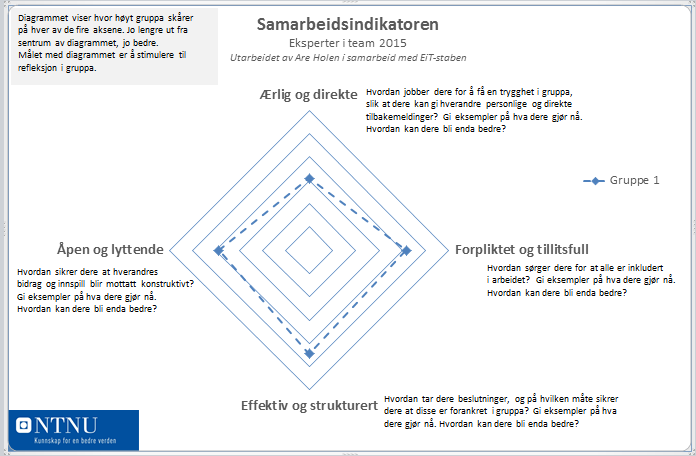
\includegraphics[width=0.45 \textwidth]{images/samarbeidsindikator_1.png}
	\label{fig:si1}
	}
\subfigure[]{
	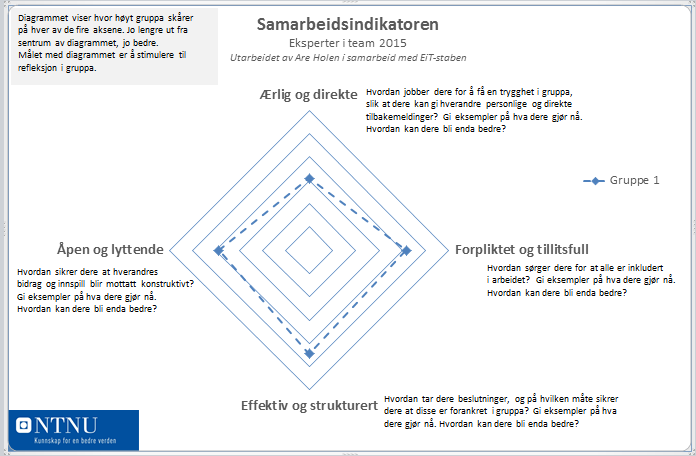
\includegraphics[width=0.45 \textwidth]{images/samarbeidsindikator_2.png}
	\label{fig:si2}
	}
\caption{Samarbeidsindikator basert på første spørreundersøkelse \protect{\ref{fig:si1}}. Samarbeidsindikator basert på siste spørreundersøkelse \protect{\ref{fig:si2}}.}
\end{figure}
Dette er vi enige i, og grunnen til denne forbedringen er at vi har hatt fokus på å være mer direkte og mer presis i tilbakemeldinger.
Teamet innså at for uklare tilbakemeldinger førte til misforståelser som førte til at stemingen i teamet ble anspent og fremdriften ble
svekket. Gjennom samarbeidet har vi utviklet oss som konfliktløserer og vi har gått fra å være todelte på enkelte områder
til så å stå sammen som et enhetlig team.


%%%
% End includes
%%%

%\newpage
%\addcontentsline{toc}{chapter}{List of Tables}
%\listoftables
%\addcontentsline{toc}{chapter}{List of Figures}
%\listoffigures
\addcontentsline{toc}{chapter}{Bibliografi}
\bibliographystyle{plain}
\thispagestyle{plain}

\begin{thebibliography}{10} %Foreløpig: oppdater dette nr som man legger til item
	
	\bibitem{tdt4856}{
		\emph{ntnu.no}
		N.P.. Web. Mar 04 2015
		<\url{http://www.ntnu.no/eit/tdt4856}>
	}
	
	\bibitem{hjulmist}{
		\emph{egenbil.no}
		N.P.. Web. Mar 04 2015
		<\url{ http://www.egenbil.no/nyttig-aa-vite/hjulmist}>
	}
		
	\bibitem{NL-skive}{
		\emph{nord-lock.com}
		N.P.. Web. Mar 04 2015
		<\url{http://www.nord-lock.com/nord-lock/wedge-locking/washers/introduction/}>
	}
	
	\bibitem{NL-hjulbolt}{
		\emph{nord-lock.com}
		N.P.. Web. Mar 04 2015
		<\url{	http://www.nord-lock.com/nord-lock/wedge-locking/wheel-nut/introduction/}>
	}
	
	\bibitem{checkpoint1}{
		\emph{cpsafety.com.au/}
		N.P.. Web. Mar 04 2015
		<\url{http://www.cpsafety.com.au/product-checkpoint.php}>
	}
		
	\bibitem{dekkslitasje-GT6}{
		\emph{pro-gmedia.com}
		N.P.. Web. Mar 04 2015
		<\url{http://s.pro-gmedia.com/videogamer/media/images/ps3/gran_turismo_6/screens/gran_turismo_6_220.jpg}>
	}

	\bibitem{FriksjonsfaktorGjenger}{
		\emph{kamax.com}
		N.P.. Web. Feb 25 2015
		<\url{http://www.kamax.com/fileadmin/user_upload/dokumente/pdf/Bolt_and_Screw_Compendium.pdf}>
	}

	\bibitem{FEManalyse}{
		Bell, Kolbein. \emph{An engineering approach to FINITE ELEMENT ANALYSIS of linear structural mechanics problems}. 1st ed. Akademika forlag, 2013. Print.
	}
	
	\bibitem{asme}{
		\emph{asme.org}
		N.P.. Web Apr 28 2015
		<\url{http://vibrationacoustics.asmedigitalcollection.asme.org/article.aspx?articleID=1840144}>
	}

	\bibitem{sagepub}{
		\emph{sagepub.com}
		N.P.. Web Apr 28 2015
		<\url{http://shm.sagepub.com/content/7/4/309.full.pdf}>
	}

	\bibitem{canbus}{
		\emph{hellanor.no}
		N.P.. Web. Mar 25 2015
		<\url{http://www.hellanor.no/filestore/PDF_filer/Teknisk_informasjon/Hella/Elektronikk/can_bus.pdf}>
	}
	
	\bibitem{adc}{
		\emph{analog.com}
		N.P.. Web. Apr 22 2015
		<\url{http://www.analog.com/en/products/analog-to-digital-converters.html}>
	}
	
	\bibitem{dsp}{
		\emph{dspguide.com}
		N.P.. Web. Apr 22 2015
		<\url{http://www.dspguide.com/ch28.htm}>
	}

	\bibitem{wheatstone}{
		\emph{electronics-tutorials.ws}
		N.P.. Web. Mar 25 2015
		<\url{http://www.electronics-tutorials.ws/blog/wheatstone-bridge.html}>
	}

	\bibitem{nyquist}{
		\emph{lavryengineering.com}
		N.P.. Web. Mar 18 2015
		<\url{http://web.archive.org/web/20060614125302/http://www.lavryengineering.com/documents/Sampling_Theory.pdf}>
	}
	
	\bibitem{PCBmail}{
		Erik Nordby \emph{Semitronic AS}.
		Personal Communications Mar 25 2015
	}
	
	\bibitem{innovasjonnorge}{
		\emph{www.innovasjonnorge.no}
		N.P.. Web. May 1 2015
		<\url{http://www.innovasjonnorge.no/no/finansiering/etablerertilskudd/#.VUPiU2Ttmkp}>
	}
	
	\bibitem{skattefunn}{
		\emph{www.forskningsradet.no}
		N.P.. Web. May 1 2015
		<\url{http://www.forskningsradet.no/prognett-skattefunn/Artikkel/Hvem_kan_fa_stotte__og_hvor_mye/1253987672197}>
	}

	\bibitem{lastebilprod-DAF}{
		\emph{daf.com/en}
		N.P.. Web. Mar 25 2015
		<\url{http://www.daf.com/en/about-daf/daf-trucks-nv/facts-and-figures}>
	}
	\bibitem{daimler}{
		\emph{daimler.com}
		N.P.. Web. Mar 25 2015
		<\url{https://www.daimler.com/company/business-units/daimler-trucks}>
	}
	
	\bibitem{MVC}{
		\emph{apple.com}
		N.P.. Web. Apr 20 2015
		<\url{https://developer.apple.com/library/mac/documentation/General/Conceptual/DevPedia-CocoaCore/MVC.html}>
	}
	
	\bibitem{firmware}{
		\emph{liteonit.eu}
		N.P.. Web. Apr 22 2015
		<\url{http://www.liteonit.eu/what_is_firmware.html}> 
	}
	
	\bibitem{embedded}{
		\emph{ece.ncsu.edu}
		N.P.. Web. Apr 20 2015
		<\url{http://www.ece.ncsu.edu/research/cas/ecs}> 
	}
	
	\bibitem{altium}{
		\emph{altium.com}
		N.P.. Web. Apr 27 2015
		<\url{http://www.altium.com/}> 
	}
	
	\bibitem{Fourier}{
		\emph{gsu.edu}
		N.P.. Web. Apr 20 2015
		<\url{http://hyperphysics.phy-astr.gsu.edu/hbase/audio/fourier.html}> 
	}

	\bibitem{aamodt94}{
		Aamodt, Agnar og Plaza, Enric. \emph{Case-Based Reasoning: Foundational Issues, Methodological Variations, and System Approaches.}
		AI Communications, Vol. 7 Nr. 1, March 1994, pp 39-59.
	}
	
\end{thebibliography}	

%\newpage
%\addcontentsline{toc}{chapter}{Appendixes} % This line may break your compilation, and may require recompiation. Not to worry though.
%\appendix
%\input{section/appendix-someAppendix}


\end{document}
